\documentclass{article}
\usepackage{graphicx} % Required for inserting images
\usepackage{cite}
\usepackage{hyperref}
\usepackage{pdfpages}

\hypersetup{
	colorlinks=true,
	linkcolor=blue,
	filecolor=magenta,      
	urlcolor=cyan,
	pdfpagemode=FullScreen,
	citecolor=black
}
\title{Data Management and Visualization Concept}
\author{Karan Kumar}

\begin{document}
	
	\maketitle
	
	\begin{center}
		\textbf{Cygnus X-1 and High Mass X-Ray Binaries}\\
		\vspace{1.5cm}
		\textbf{Target Audience: General Public and Science Communicators}
		\textbf{Publication: }
		
	\end{center}
	
	This data concept is part of my Masters' Thesis on High-Mass X-Ray Binaries (HMXBs) in the Galaxy. These are stars made of a massive star and a black hole (or neutron star) that orbit around each other. My thesis also involves using archive data from the GAIA space telescope. I searched through the literature to find these stars specifically with GAIA. There are many catalogues, me and my thesis supervisor selected \cite{Neumann} and crossed references with \cite{Carretero} which has the most up-to-date information about HMXBs, each star as a unique GAIA identifier which I can use to query the position of stars from the GAIA database, which is free to use for anyone. The catalogue is free to use and I have provided the link to the dataset. \href{http://astro.uni-tuebingen.de/~xrbcat/}{link to the catalgoue}
	The .csv file I share has all the information about the stars including spectral type which I color coded by hand. There are also additional columns in the file about velocities, mass and proper motion but these aren't required to recreate the data.
	To replicate the data you need these columns 
	\begin{enumerate}
		\item ra :right ascension
		\item dec: declination
		\item l : galactic longitude
		\item b : galactic latitude
		\item d : distance to object 
		\item SpColor: Spectral Type Color		 
	\end{enumerate}
	The first part of my thesis was to visualize where these stars are in the galaxy, the catalogue and GAIA let you plot the 2D position of each star in galactic coordinates. 
	\newline
	My data story was to show the public where exactly these stars are in the galaxy. I want to show simple maps of the stars in the galaxy using coordinate systems that other astronomers use; figure 1 in the poster is a galactic map in unit degrees to represent the 2D position of each star in the catalogue, the map is an edge on view of the galaxy. Stars also have Z-component which represents the height above or below the midplane of the galaxy, which is represented in figure 2 in the poster. Unlike figure 1, the height also depends on the distance to the star from us, stars closer to us will have a smaller projected height for the same galactic latitude (I show this in the code). So I chose to show the height over galactic longitude so the reader has a constant axis to refer to. 
	\newline
	\textbf{Cygnus X-1}: This is one of the most famous and well studied HMXBs ever since its discovery in 1964. I wanted to show what a typical HMXB could look like with a simple drawing. I scaled the image with respect to earth's distance to the sun And I tried to give everything in scales the general public could understand such as 1AU ~ 150 million Km or mass and radii in solar values. I also emphasized the location of Cygnus X-1 so the reader was always engaged with the system while viewing the poster. The facts about the system come from \cite{CygnusX-1}
	% I also only plot stars with confident distance to us, some stars aren't resolved well by GAIA because of noise or an obstructed view, by plotting stars I'm confident in I can clearly show where
	
	
	\subsection{Radial velocity Spectrometer}
	Data compliments $G_{BP} , G_RP$
	The \textit{GAIA} Radial Velocity Spectrometer (RVS) offers high resolution, narrow band spectra for 33.8 million sources in the sky \cite{GAIA}. The RVS measures the doppler shift of objects with its line of sight to determine the radial velocity as well as measure a radial veloicty magnitude for the brightest stars $G_{RVS} \leq 14 $. THE RVS obtains the radial velocity by measuring the spectra between 845-872 nm which covers the Ca II triplet emission line. The Ca II triplet is also used to measure metallically, temperatures and luminosity. CITE GAIA,  Sartoretti.
	\subsection{Photometric Instrument}
	The Photometric Instrument uses the same focal plane and telescope as the Astrometric intrsument to measure the spectral energy distribution for all objects in the sky at a given epoch \cite{GAIA}. Light enters the instrument and is split by two silica prisms which seperate the light into the Blue photometer (BP) at 330-680 nm and the red photometer (RP) at 640-1050nm. NEED MORE INFO
	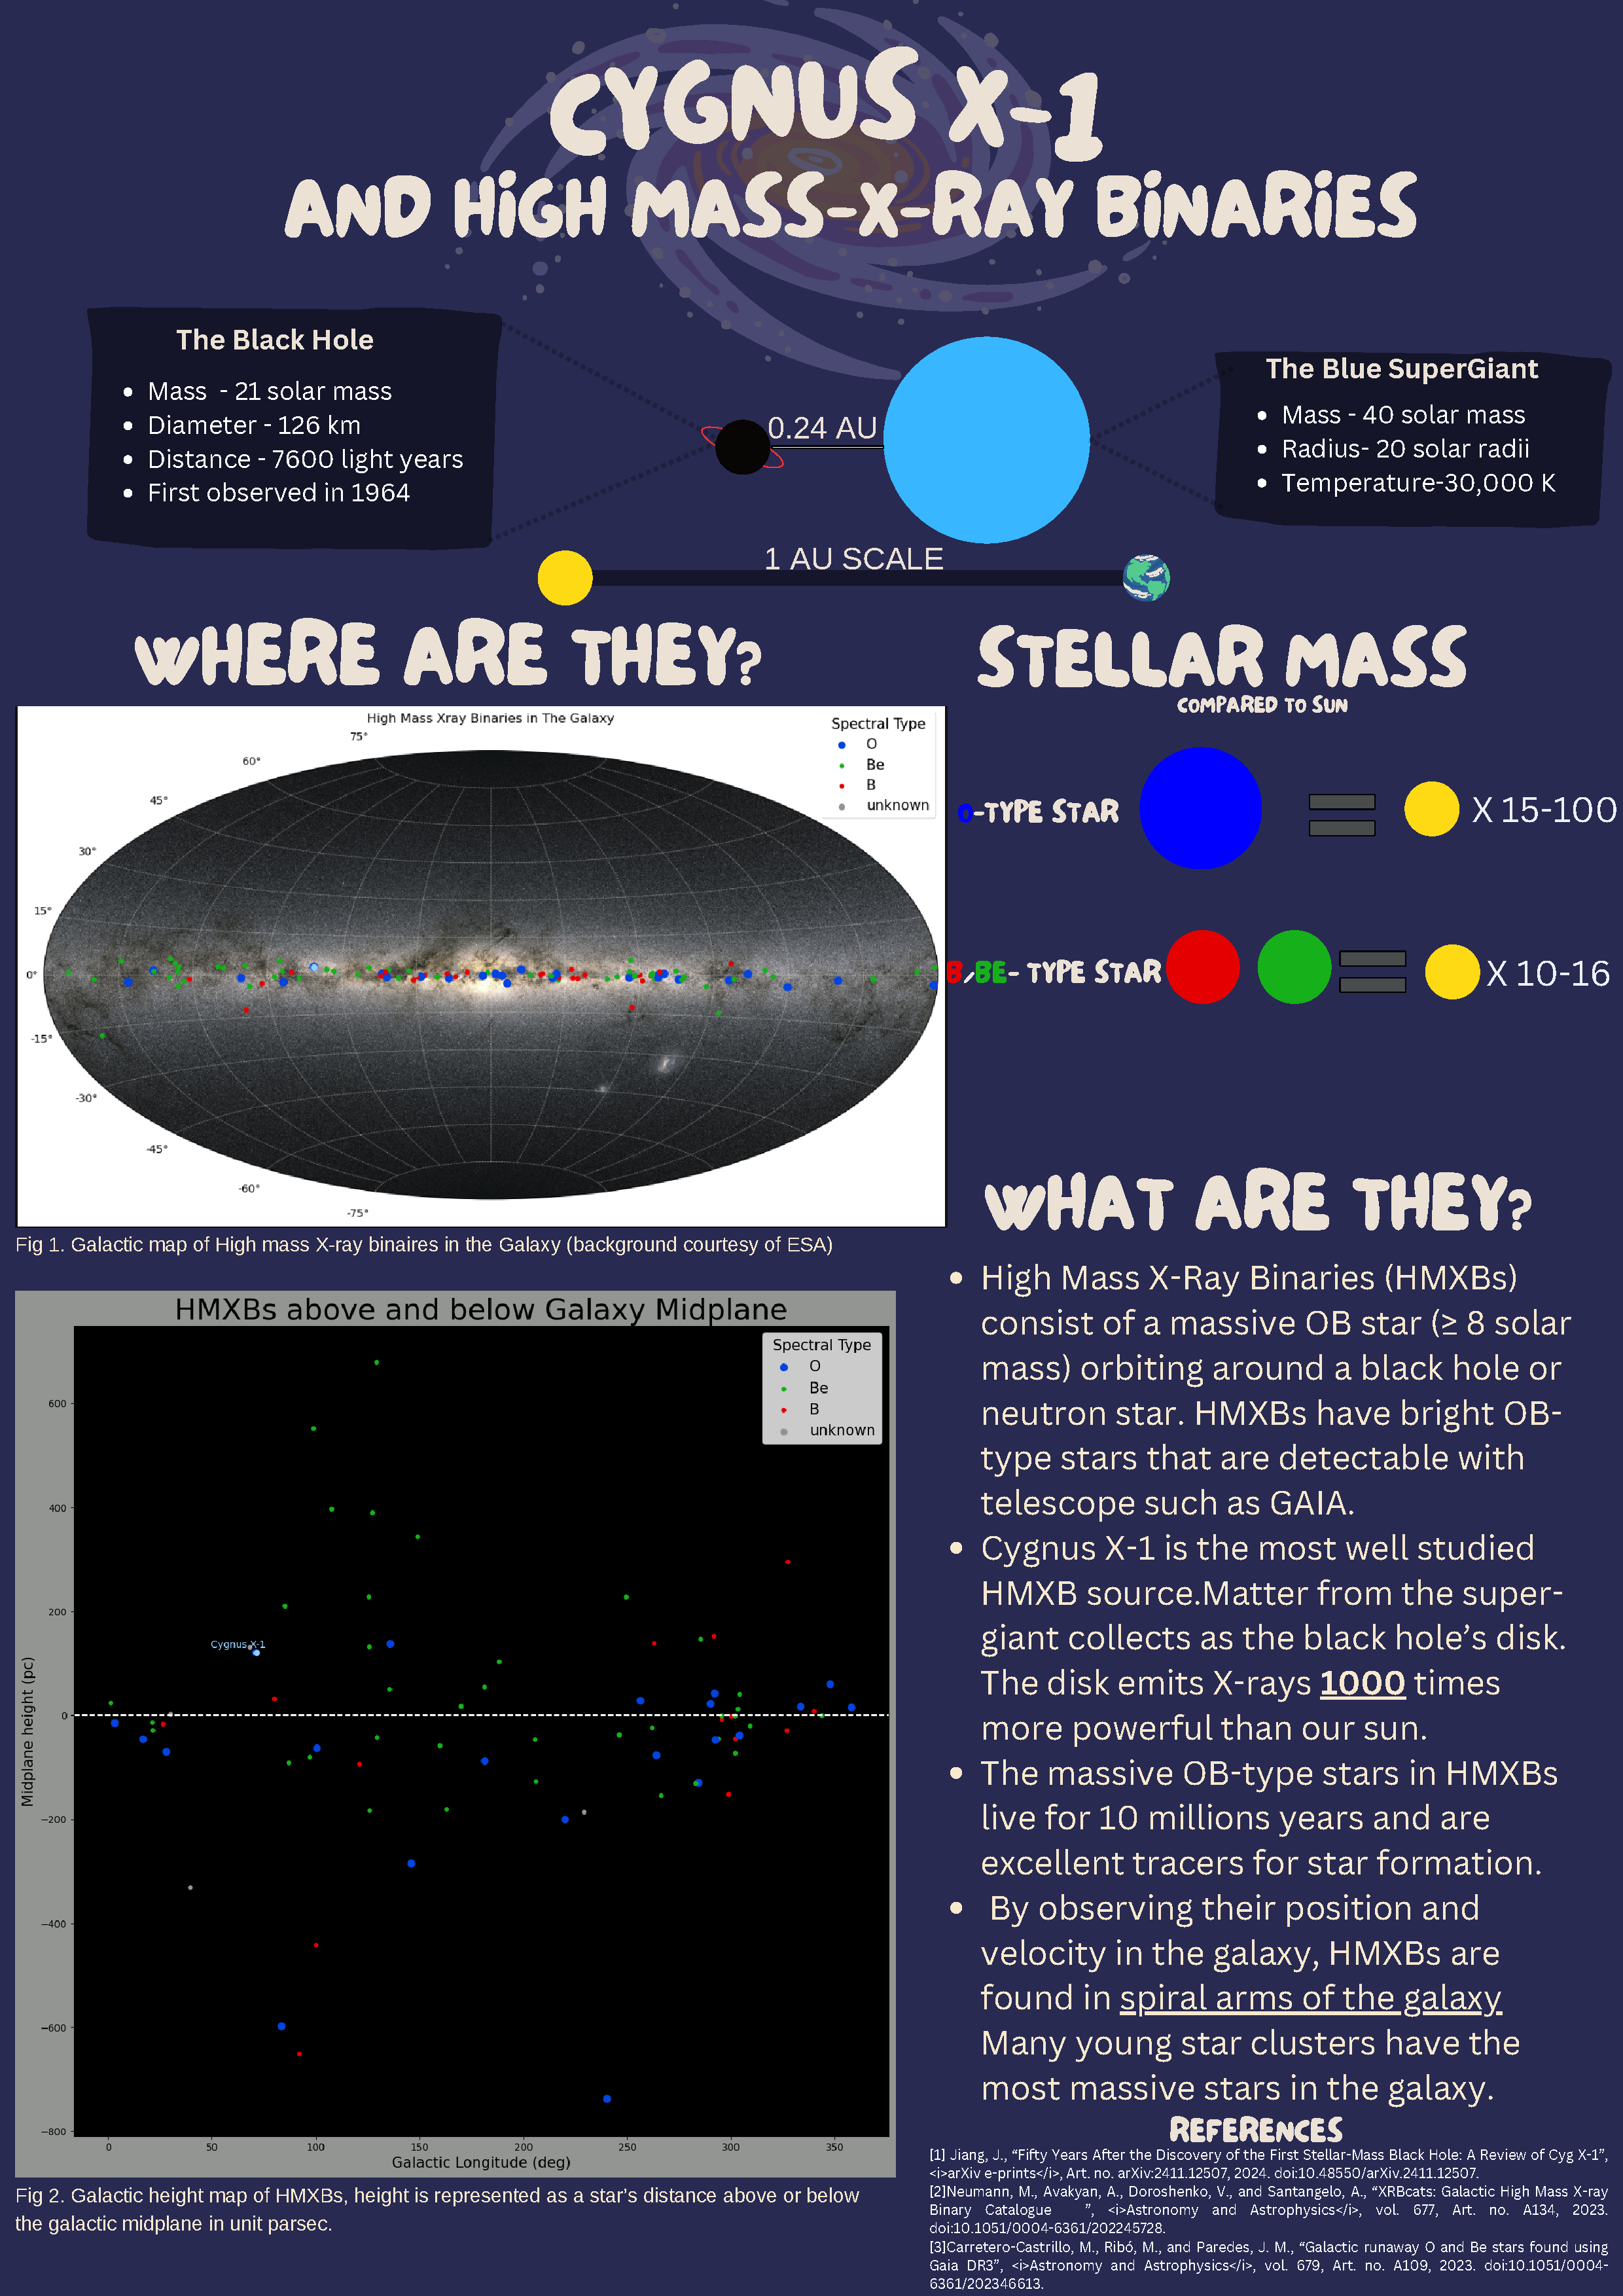
\includepdf[pages=-]{Cygnus X-1.pdf}
	\bibliography{Bibliography.bib}
	\bibliographystyle{plain}
\end{document}
